\documentclass[11pt]{article}

% if you need to pass options to natbib, use, e.g.:
%\PassOptionsToPackage{numbers}{natbib}
\usepackage[colorlinks,linkcolor=blue,filecolor=blue,citecolor=magenta,urlcolor=blue]{hyperref}
\usepackage{bm,amsmath,amsthm,amssymb,multicol,algorithmic,algorithm,enumitem,graphicx,subfigure}
\usepackage{xargs}
\usepackage{stmaryrd}
\usepackage{natbib}

% ready for submission
\usepackage{neurips_2021}
\def\M{\mathcal{M}}
\def\A{\mathcal{A}}
\def\Z{\mathcal{Z}}
\def\S{\mathcal{S}}
\def\D{\mathcal{D}}
\def\R{\mathcal{R}}
\def\P{\mathcal{P}}
\def\K{\mathcal{K}}
\def\E{\mathbb{E}}
\def\F{\mathfrak{F}}
\def\l{\boldsymbol{\ell}}

\newtheorem{Fact}{Fact}
\newtheorem{Lemma}{Lemma}
\newtheorem{Prop}{Proposition}
\newtheorem{Theorem}{Theorem} 
\newtheorem{Def}{Definition}
\newtheorem{Corollary}{Corollary}
\newtheorem{Conjecture}{Conjecture}
\newtheorem{Property}{Property}
\newtheorem{Observation}{Observation}
\newtheorem{Exa}{Example}
\newtheorem{assumption}{H\!\!}
\newtheorem{Remark}{Remark}
\newtheorem*{Lemma*}{Lemma}
\newtheorem*{Theorem*}{Theorem}
\newtheorem*{Corollary*}{Corollary}
 
\newcommand{\eqsp}{\;}
\newcommand{\beq}{\begin{equation}}
\newcommand{\eeq}{\end{equation}}
\newcommand{\eqdef}{\mathrel{\mathop:}=}
\def\EE{\mathbb{E}}
\newcommand{\norm}[1]{\left\Vert #1 \right\Vert}
\newcommand{\pscal}[2]{\left\langle#1\,|\,#2 \right\rangle}
\def\major{\mathsf{M}}
\def\rset{\ensuremath{\mathbb{R}}}

\begin{document}
\title{Sparsified Distributed Adaptive Learning \\
with Error Feedback}

\author{
Xiaoyun Li \\
  Cognitive And Computing Lab\\
  Baidu Research\\
  Beijing, USA \\
  \texttt{xiaoyun@baidu.com} 
   \And
  Belhal Karimi \\
  Cognitive And Computing Lab\\
  Baidu Research\\
  Beijing, China \\
  \texttt{v_karimibelhal@baidu.com} 
   \And
  Ping Li \\
  Cognitive And Computing Lab\\
  Baidu Research\\
  Beijing, China \\
  \texttt{liping@baidu.com} \\
}

\date{\today}

\maketitle

\begin{abstract}
In this paper, we present a novel optimization algorithm for single-machine and distributed learning, based on sparsification and error feedback techniques to lighten the communications between a central server and distributed workers.
The method we introduce builds on the adaptivity of the AMSGrad method for nonconvex optimization, and includes a TopK operation to alleviate any communication bottleneck between a large amount of devices and a central computing server, combined with a correction of the natural bias induced by the latter compression operator.
Despite the sparsity induced by our algorithm, we show that \algo reaches a stationary point in $\mathcal{O}(1/ \sqrt{T})$ iterations, matching that of state-of-the-art single-machine methods.
We illustrate on benchmark datasets the effectiveness of our method both under the single-machine and distributed settings.
\end{abstract}

\section{Introduction}\label{sec:introduction}

Deep neural network has achieved the state-of-the-art learning performance on numerous AI applications, e.g., computer vision~\cite{Proc:GAN_NIPS14,Proc:Resnet_CVPR16,CV_review18}, Natural Language Processing~\cite{Proc:Graves_ICASSP13,NLP_review18,sentiment_review18}, Reinforcement Learning~\cite{Arxiv:MnihKSGAWR13,AlphaGo_17} and recommendation systems~\cite{Proc:Covington_2016,Article:Wei_2017}. With the increasing size of both data and deep networks, standard single machine training confronts with at least two major challenges:
\begin{itemize}
    \item Due to the limited computing power of a single machine, it would take a long time to process the massive number of data samples---training would be slow.
  
    \item In many practical scenarios, data are typically stored in multiple servers, possibly at different locations, due to the storage constraints (massive user behavior data, Internet images, etc.) or privacy reasons~\cite{Proc:Chang18}. Transmitting data might be costly.
\end{itemize}
\textit{Distributed learning} framework~\cite{Proc:Dean_NIPS12} has been a common training strategy to tackle the above two issues. For example, in centralized distributed stochastic gradient descent (SGD) protocol, data are located at $N$ local nodes, at which the gradients of the model are computed in parallel. In each iteration, a central server aggregates the local gradients, updates the global model, and transmits back the updated model to the local nodes for subsequent gradient computation. As we can see, this setting naturally solves aforementioned issues: 1) We use $N$ computing nodes to train the model, so the time per training epoch can be largely reduced; 2) There is no need to transmit the local data to central server. Besides, distributed training also provides stronger error tolerance since the training process could continue even one local machine breaks down. As a result of these advantages, there has been a surge of study and applications on distributed systems~\cite{boyd2011distributed,nedic2009distributed,duchi2011dual,Arxiv:Goyal17,hong2017prox,lu2019gnsd,koloskova2019decentralized}.

Among many optimization strategies, SGD is still the most popular prototype in distributed training for its simplicity and effectiveness~\cite{chilimbi2014project,Proc:Agrawal_NIPS19,mikami2018massively}. Yet, when the deep learning model is very large, the communication between local nodes and central server could be expensive. Burdensome gradient transmission would slow down the whole training system, or even be impossible because of the limited bandwidth in some applications. Thus, reducing the communication cost in distributed SGD has become an active topic, and an important ingredient of large-scale distributed systems (e.g.~\cite{Proc:Seide14}). Solutions based on quantization, sparsification and other compression techniques of the local gradients are proposed, e.g.,~\cite{alistarh2017qsgd,wen2017terngrad,wangni2018gradient,stich2018sparsified,aji2017sparse,bernstein2018signsgd,de2017understanding,yang2019swalp,Proc:Ivkin_NIPS19}. As one would expect, in most approaches, there exists a trade-off between compression and model accuracy. In particular, larger bias of the compressed gradients usually brings more significant performance downgrade. Interestingly, \cite{karimireddy2019error} shows that the technique of \textit{error feedback} is able to remedy the issue of such biased compressors, achieving same convergence rate and learning performance as full-gradient SGD.


On the other hand, in recent years, adaptive optimization algorithms (e.g. AdaGrad~\cite{Duchi10-adagrad}, Adam~\cite{kingma2014adam} and AMSGrad~\cite{reddi2019convergence}) have become popular because of their superior empirical performance. These methods use different implicit learning rates for different coordinates that keep changing adaptively throughout the training process, based on the learning trajectory. In many learning problems, adaptive methods have been shown to converge faster than SGD, sometimes with better generalization as well. However, the body of literature that combines adaptive methods with distributed training is still very limited. In this papar, we propose a distributed optimization algorithm with AMSGrad as the backbone, along with Top-$k$ sparsification to reduce the communication cost.

\subsection{Our contributions}

We develop a simple optimization leveraging the adaptivity of AMSGrad, and the computational virtue of TopK sparsification, for tackling a large finite-sum of nonconvex objective functions.

Our technique is shown to be both theoretically and empirically effective under \emph{the classical centralized setting} and \emph{the distributed setting}.

In this contribution, 
\begin{itemize}
\item We derive a sparsified AMSGrad with error feedback, called \algo, with a single machine and provide its decentralized counter part.
\item We provide a non-asymptotic convergence rate under each setting,
\item We highlight the effectiveness of both methods through several numerical experiments
\end{itemize}


\section{Related Work}\label{sec:related}

\subsection{Communication-efficient distributed SGD}

\paragraph{Quantization.} As we mentioned before, SGD is the most commonly adopted optimization method in distributed training of deep neural nets. To reduce the expensive communication in large-scale distributed systems, extensive works have considered various compression techniques applied to the gradient transaction procedure. The first strategy is quantization. \cite{Proc:8-bit_ICLR16} condenses 32-bit floating numbers into 8-bits when representing the gradients. \cite{Proc:Seide14,bernstein2018signsgd,karimireddy2019error,Proc:Bernstein_ICLR19} use the extreme 1-bit information (sign) of the gradients, combined with tricks like momentum, majority vote and memory. Other quantization-based methods include QSGD~\cite{alistarh2017qsgd,Proc:Wu_ICML18,Proc:Zhang_ICML17} and LPC-SVRG~\cite{Proc:Yu_AISTATS19}, leveraging unbiased stochastic quantization. The saving in communication of quantization methods is moderate: for example, 8-bit quantization reduces the cost to 25\% (compared with 32-bit full-precision). Even in the extreme 1-bit case, the largest compression ratio is around $1/32\approx 3.1\%$. 

\paragraph{Sparsification.} Gradient sparsification is another popular solution which may provide higher compression rate. Instead of commuting the full gradient, each local worker only passes a few coordinates to the central server and zeros out the others. Thus, we can more freely choose higher compression ratio (e.g., 1\%, 0.1\%), still achieving impressive performance in many applications~\cite{Proc:Lin_ICLR18}. Stochastic sparsification methods, including uniform sampling and magnitude based sampling~\cite{wangni2018gradient}, select coordinates based on some sampling probability yielding unbiased gradient compressors. Deterministic methods are simpler, e.g., Random-$k$, Top-$k$~\cite{stich2018sparsified,shi2019convergence} (selecting $k$ elements with largest magnitude), Deep Gradient Compression~\cite{Proc:Lin_ICLR18}, but usually lead to biased gradient estimation. In~\cite{Proc:Ivkin_NIPS19}, the central server identifies heavy-hitters from the count-sketch~\cite{Proc:Charikar_ICALP02} of the local gradients, which can be regarded as a noisy variant of Top-$k$ strategy. More applications and analysis of compressed distributed SGD can be found in~\cite{jiang2018linear,Proc:Shen_ICML18,alistarh2018convergence,Proc:Basu_NIPS19,Proc:Jiang_SIGMOD18}, among others.

\paragraph{Error Feedback.} Biased gradient estimation, which is a consequence of many aforementioned methods (e.g., signSGD, Top-$k$), undermines the model training, both theoretically and empirically, with slower convergence and worse generalization. The technique of \textit{error feedback} is able to ``correct for the bias'' and fix the problems. In this procedure, the difference between the true stochastic gradient and the compressed one is accumulated locally, which is then added back to the local gradients in later iterations. \cite{stich2018sparsified,karimireddy2019error} prove the $\mathcal O(\frac{1}{T})$ and $\mathcal O(\frac{1}{\sqrt T})$ convergence rate of EF-SGD in strongly convex and non-convex setting respectively, matching the rates of vanilla SGD~\cite{nemirovski2009robust,ghadimi2013stochastic}.


\subsection{Adaptive optimization}

In each SGD update, all the gradient coordinates share a same learning rate, either constant or decreasing over iterations. Adaptive optimization methods cast different learning rate on each dimension. AdaGrad~\cite{Duchi10-adagrad} divides the gradient element-wisely by $\sqrt{\sum_{t=1}^T g_{t}^2}\in \mathbb R^d$, where $g_{t}\in \mathbb R^d$ is the gradient vector at time $t$ and $d$ is the model dimensionality. Thus, it intrinsically assigns different learning rates to different coordinates throughout the training---elements with smaller previous gradient magnitude tend to move a larger step. AdaGrad has been shown to perform well especially under some sparsity structure. AdaDelta~\cite{Proc:adadelta} and Adam~\cite{kingma2014adam} introduce momentum and moving average of second moment estimation into AdaGrad which lead to better performance. AMSGrad~\cite{reddi2019convergence} fixes the potential convergence issue of Adam, which will serve as the prototype in this paper. We present the psudocode in Algorithm . In general, adaptive optimization methods are easier to tune in practice, and usually exhibit faster convergence than SGD. Thus, they have been widely used in training deep learning models in language and computer vision applications, e.g.,~\cite{,Arxiv:Choi_2019,Proc:LAMB_ICLR20,Arxiv:Zhang_ICLR21}. In distributed setting, the work~\cite{nazari2019dadam} proposes a decentralized system in online optimization. However, communication efficiency is not considered. The recent work~\cite{chen2020quantized} is the most relevant to our paper. Yet, their method is based on Adam, and requires every local node to store a local estimation of first and second moment, thus being less efficient. We will present more detailed comparison in Section~\ref{sec:main}.


\section{Communication-Efficient Adaptive Optimization}\label{sec:main}

Most modern machine learning tasks can be casted as a large finite-sum optimization problem written as:
\begin{equation}\label{eq:opt}
\min \limits_{\theta \in \Theta} \frac{1}{n} \sum_{i=1}^n f_i(\theta)
\end{equation}
where $n$ denotes the number of workers, $f_i$ represents the average loss for worker $i$ and $\theta$ the global model parameter taking value in $\Theta$, a subset of $\mathbb{R}^d$.



Some related work:


\citep{karimireddy2019error} develops variant of signSGD (as a biased compression schemes) for distributed optimization. Contributions are mainly on this error feedback variant.
In \citep{shi2019convergence}, the authors provide theoretical results on the convergence of sparse Gradient SGD for distributed optimization (we want that for AMS here).
\citep{stich2018sparsified} develops a variant of distributed SGD with sparse gradients too. Contributions include a memory term used while compressing the gradient (using top k for instance). Speeding up the convergence in $\frac{1}{T^3}$.
% \url{https://arxiv.org/pdf/1901.09847.pdf}
% \url{https://pdfs.semanticscholar.org/8728/dee89906022c1d4f5c1de1233c3f65ab92f2.pdf?_ga=2.152244026.2027005181.1606271153-15127215.1603945483}
% \url{https://proceedings.neurips.cc/paper/2018/file/b440509a0106086a67bc2ea9df0a1dab-Paper.pdf}

Consider standard synchronous distributed optimization setting. AMSGrad is used as the prototype, and the local workers is only in charge of gradient computation.


\subsection{TopK AMSGrad with Error Feedback}




The key difference (and interesting part) of our TopK AMSGrad compared with the following arxiv paper ``Quantized Adam''\url{https://arxiv.org/pdf/2004.14180.pdf} is that, in our model only gradients are transmitted. In ``QAdam'', each local worker keeps a local copy of moment estimator $m$ and $v$, and compresses and transmits $m/v$ as a whole. Thus, that method is very much like the sparsified distributed SGD, except that $g$ is changed into $m/v$. In our model, the moment estimates $m$ and $v$ are computed only at the central server, with the compressed gradients instead of the full gradient. This would be the key (and difficulty) in convergence analysis.


\begin{algorithm}[H]
\caption{\algo\ for Distributed Learning} \label{alg:sparsams}
\begin{algorithmic}[1]

\STATE \textbf{Input}: parameter $\beta_1$, $\beta_2$, learning rate $\eta_t$. 
\STATE Initialize: central server parameter $\theta_{0} \in \Theta \subseteq \mathbb R^d$; $e_{1,i}=0$ the error accumulator for each worker; sparsity parameter $k$; $n$ local workers; $m_0=0$, $v_0=0$, $\hat v_0=0$

\FOR{$t=1$ to $T$}

\STATE\textbf{parallel for worker $i \in [n]$ do}:
\STATE\quad  Receive model parameter $\theta_{t}$ from central server
\STATE\quad  Compute stochastic gradient $g_{t,i}$ at $\theta_t$
\STATE\quad  Compute $\tilde g_{t,i}=TopK(g_{t,i}+e_{t,i},k)$ \label{line:topk} 
\STATE\quad  Update the error $e_{t+1,i}=e_{t,i}+g_{t,i}-\tilde g_{t,i}$
\STATE\quad  Send $\tilde g_{t,i}$ back to central server
\STATE \textbf{end parallel}

\STATE \textbf{Central server do:}
\STATE $\bar g_{t}=\frac{1}{n}\sum_{i=1}^N \tilde g_{t,i}$
\STATE $m_t=\beta_1 m_{t-1}+(1-\beta_1)\bar g_t$
\STATE $v_t=\beta_2 v_{t-1}+(1-\beta_2)\bar g_t^2$
\STATE $\hat v_t=\max(v_t,\hat v_{t-1})$ \label{line:v}
\STATE Update global model $\theta_{t+1}=\theta_{t}-\eta_t\frac{m_t}{\sqrt{\hat v_t+\epsilon}}$

\ENDFOR
\end{algorithmic}
\end{algorithm}


\subsection{Convergence Analysis}

Several mild assumptions to make: Nonconvex and smooth loss function, unbiased stochastic gradient, bounded variance of the gradient, bounded norm of the gradient, control of the distance between the true gradient and its sparse variant.

Check \citep{chen2020quantized} starting with single machine  and extending to distributed settings (several machines).


Under the distributed setting, the goal is to derive an upper bound to the second order moment of the gradient of the objective function at some iteration $T_f \in [1, T]$.

\subsection{Mild Assumptions}
We begin by making the following assumptions.

\begin{assumption}\label{ass:smooth}(Smoothness)
For $i \in \inter$, $f_i$ is  L-smooth: $\norm{\nabla f_i (\theta) - \nabla f_i (\vartheta)} \leq L \norm{\theta-\vartheta}$.
\end{assumption}

\begin{assumption}\label{ass:boundgrad}(Unbiased and Bounded gradient \textbf{per worker})
For any iteration index $t >0$ and worker index $i \in \inter$, the stochastic gradient is unbiased and bounded from above: $\EE[g_{t,i}] = \nabla f_i(\theta_t)$ and $\norm{g_{t,i}} \leq G_i$.
\end{assumption}

\begin{assumption}\label{ass:quant}(Bounded variance \textbf{per worker})
For any iteration index $t >0$ and worker index $i \in \inter$, the variance of the noisy gradient is bounded: $\EE[|g_{t,i} - \nabla f_i(\theta_t)|^2] < \sigma_i^2$.
\end{assumption}

Denote by $Q(\cdot)$ the quantization operator Line~\ref{line:topk} of Algorithm~\ref{alg:sparsams}, which takes as input a gradient vector and returns a quantized version of it, and note $\tilde{g} \eqdef Q(g)$.
Assume that
\begin{assumption}\label{ass:var}(Bounded Quantization)
For any iteration $t >0$, there exists a constant $0 < q < 1$ such that $\norm{g_{t,i} - \tilde{g}_{t,i}} \leq q \norm{g_{t,i}}$, where $g_{t,i}$ is the stochastic gradient computed at iteration $t$ for worker $i$ and $\tilde{g}_{t,i}$ is its quantized counterpart. \textcolor{red}{(high $q$ means large quantization so loss of precision on the true gradient)}
\end{assumption}


Denote for all $\theta \in \Theta$:
\begin{equation}\label{eq:obj}
f(\theta) \eqdef  \frac{1}{n} \sum_{i=1}^n f_i(\theta) \, ,
\end{equation} 
where $n$ denotes the number of workers.



\subsection{Intermediary Lemmas}

\begin{Lemma}\label{lem:bound}
Under Assumption~\ref{ass:boundgrad} and Assumption~\ref{ass:var} we have for any iteration $t >0$:

\begin{equation}
\norm{m_t}^2 \leq (q^2+1) G^2 \quad \textrm{and} \quad \hat v_t \leq (q^2+1) G^2
\end{equation}
where $m_t$ and $\hat v_t=\max(v_t,\hat v_{t-1})$ are defined Line~\ref{line:v} of Algorithm~\ref{alg:sparsams} and $G^2 = \frac{1}{n}\sum_{i=1}^N  G_{i}^2$.
\end{Lemma}


\begin{Lemma}\label{lem:lemma1}
Under A\ref{ass:smooth} to A\ref{ass:var}, with a decreasing sequence of stepsize $\{\eta_t\}_{t>0}$, we have:

\begin{equation}
-\eta_{t+1}\EE[\pscal{\nabla f(\theta_t)}{(\hat{V}_{t+1} + \epsilon \mathsf{I_d})^{-1/2} \bar{g}_t}] \leq - \frac{\eta_{t+1}}{2}  (\epsilon + \frac{(q^2+1)G^2}{1 - \beta_2})^{-\frac{1}{2}} \EE[\norm{\nabla f(\theta_t)}^2] +q^2 \frac{G^2 \eta_{t+1}}{\epsilon 2n^2}
\end{equation}
where $ \mathsf{I_d}$ is the identity matrix, $\hat{V_t}$ the diagonal matrix which diagonal entries are $\hat v_t=\max(v_t,\hat v_{t-1})$ defined Line~\ref{line:v} of Algorithm~\ref{alg:sparsams} and $\bar{g}_t$ is the aggregation of all \textbf{quantized} gradients from the workers.
\end{Lemma}

\begin{Lemma}\label{lem:lemma2}
Under A\ref{ass:smooth} to A\ref{ass:var}, with a decreasing sequence of stepsize $\{\eta_t\}_{t>0}$, we have:

\begin{equation}
\begin{split}
\EE[f(\theta_{t+1}) - f(\theta_{t}) ] \leq &   - \frac{\eta_{t+1}(1-\beta_1)}{2}  (\epsilon + \frac{(q^2+1)G^2}{1 - \beta_2})^{-\frac{1}{2}} \EE[\norm{\nabla f(\theta_t)}^2] +q^2 \frac{G^2 \eta_{t+1}}{\epsilon 2n^2} \\
&- \eta_{t+1} \beta_1\EE[\pscal{\nabla f(\theta_{t-1})}{(\hat{V}_{t} + \epsilon \mathsf{I_d})^{-1/2} m_{t}}]\\
& +  \left(\frac{L}{2} + \beta_1 L \right) \norm{\theta_t - \theta_{t-1}}^2\\
&+   \eta_{t+1} G^2 \EE[\sum_{j=1}^d \left[(\hat{v}^j_{t+1} + \epsilon )^{-1/2} - (\hat{v}^j_{t} + \epsilon )^{-1/2}  \right] ]
\end{split}
\end{equation}
where $d$ denotes the dimension of the parameter vector
\end{Lemma}


\textbf{Decentralized Workers Setting:}

The main theorem in the decentralized setting reads:

\begin{Theorem}\label{thm:mainmultiple}
Under A\ref{ass:smooth} to A\ref{ass:var}, with a constant stepsize $\eta_t = \eta = \frac{L}{\sqrt{\maxiter}}$, the sequence of iterates $\{\theta_t\}_{t>0}$ output from Algorithm~\ref{alg:sparsams} satisfies:

\begin{equation}
\begin{split}
 \frac{1}{\maxiter}\sum_{t=0}^{\maxiter -1} \EE[\norm{\nabla f(\theta_t)}^2] \leq \frac{\EE[ f(\theta_{0}) - f(\theta_{\maxiter})]}{L \Delta_1 \sqrt{\maxiter}} + 
d\frac{L \Delta_3}{\Delta_1 \sqrt{\maxiter}}  + \frac{\Delta_2}{\eta \Delta_1\maxiter} +\frac{1-\beta_1}{\Delta_1}  \epsilon^{-\frac{1}{2}} \sqrt{(q^2+1)}G^2 
\end{split}
\end{equation}


where 
\begin{equation}
\begin{split}
\Delta_1 & \eqdef \frac{(1-\beta_1)}{2} (\epsilon + \frac{(q^2+1)G^2}{1 - \beta_2})^{-\frac{1}{2}} \quad \textrm{,} \quad \Delta_2 \eqdef q^2 + \sum_{k=t+1}^\infty  \beta_1^{k-t+2}\frac{G^2 }{\epsilon 2n^2}\\
\Delta_3 &\eqdef \left(\frac{L}{2} + 1+ \frac{\beta_1L}{1-\beta_1} \right) (1-\beta_2)^{-1} (1 - \frac{\beta_1^{2}}{\beta_2})^{-1}
\end{split}
\end{equation}
\end{Theorem}

We remark from this bound in Theorem~\ref{thm:mainmultiple}, that the more quantization we apply to our gradient vectors ($q \uparrow$), the larger the upper bound of the stationary condition is, \ie the slower the algorithm is. 
This is intuitive as using compressed quantities will definitely impact the algorithm speed.
We will observe in the numerical section below that a trade-off on the level of quantization $q$ can be found to achieve similar speed of convergence with less computation resources used throughout the training.





\textbf{Single Machine Setting:}

\begin{Theorem}\label{thm:mainsingle}
Under A\ref{ass:smooth} to A\ref{ass:var}, with a constant stepsize $\eta_t = \eta = \frac{L}{\sqrt{\maxiter}}$, the sequence of iterates $\{\theta_t\}_{t>0}$ output from Algorithm~\ref{alg:sparsamssingle} satisfies:

\ \begin{align}
 \frac{1}{\maxiter}\sum_{t=0}^{\maxiter -1} \EE[\norm{\nabla f(\theta_t)}^2]  \leq &
 \frac{\EE[f(\theta_{0}) - f(\theta_{\maxiter})]}{\maxiter(\eta\frac{1}{\sqrt{G^2+\epsilon}} + q )} + \eta^2 G^2\frac{L}{2} \frac{q^2+1}{\epsilon(\eta\frac{1}{\sqrt{G^2+\epsilon}} + q)} \\
 & + \eta G^2 \frac{q\sqrt{q^2+1}}{\sqrt{\epsilon}(1-q)(\eta\frac{1}{\sqrt{G^2+\epsilon}} + q)}  +  \frac{G^2}{(\eta\frac{1}{\sqrt{G^2+\epsilon}} + q)} \left(\frac{q}{1-q}\right)^2 \left[ \frac{L}{2}q^2 + 1 \right]
  \end{align}
\end{Theorem}

\section{Sequential Model}

Single machine method

\begin{algorithm}[H]
\caption{\algo\ : Single machine setting} \label{alg:sparsamssingle}
\begin{algorithmic}[1]

\STATE \textbf{Input}: parameter $\beta_1$, $\beta_2$, learning rate $\eta_t$. 
\STATE Initialize: central server parameter $\theta_{1} \in \Theta \subseteq \mathbb R^d$; $e_{1}=0$ the error accumulator; sparsity parameter $k$; $m_0=0$, $v_0=0$, $\hat v_0=0$

\FOR{$t=1$ to $T$}
\STATE  Compute stochastic gradient $g_{t} = g_{t,i_t}$ at $\theta_t$ for randomly sampled index $i_t$\label{line:stochgrad} 
\STATE  Compute $\tilde g_{t}=TopK(g_{t}+e_{t},k)$ \label{line:topksingle} 
\STATE  Update the error $e_{t+1}=e_{t}+g_{t}-\tilde g_{t}$
\STATE $m_t=\beta_1 m_{t-1}+(1-\beta_1)\tilde g_t$
\STATE $v_t=\beta_2 v_{t-1}+(1-\beta_2)\tilde g_t^2$
\STATE $\hat v_t=\max(v_t,\hat v_{t-1})$ \label{line:vsingle}
\STATE Update global model $\theta_{t+1}=\theta_{t}-\eta_t\frac{m_t}{\sqrt{\hat v_t+\epsilon}}$

\ENDFOR
\end{algorithmic}
\end{algorithm}


%We first define multiple auxiliary sequences. For the first moment, define
%
%\begin{align*}
%    &\bar m_t=m_t+\mathcal E_t,\\   
%    &\mathcal E_t=\beta_1\mathcal E_{t-1}+(1-\beta_1)(e_{t+1}-e_t),
%\end{align*}
%such that 
%\begin{align*} 
%    \bar m_t&=\bar m_t+\mathcal E_t\\
%    &=\beta_1(m_t+\mathcal E_t)+(1-\beta_1)(\bar g_t+e_{t+1}-e_1)\\
%    &=\beta_1\bar m_{t-1}+(1-\beta_1)g_t.
%\end{align*}


Let $m_t'$ be the first moment moving average of standard AMSGrad using full gradients. $m_t'=(1-\beta_1)\sum_{i=1}^k\beta_1^{t-i} g_t$. Denote
\begin{align*}
    a_t=\frac{m_t}{\sqrt{\hat v_t+\epsilon}},\quad a_t'=\frac{m_t'}{\sqrt{\hat v_t'+\epsilon}}.
\end{align*}
Define the sequence
\begin{align*}
    \mathcal E_{t+1}=\mathcal E_t+a_t'-a_t,
\end{align*}
such that the auxiliary model
\begin{align*}
    \theta_{t+1}'&\eqdef\theta_{t+1}-\eta \mathcal E_{t+1}\\
    &=\theta_t-\eta a_t-\eta\mathcal E_{t+1}\\
    &=\theta_t-\eta a_t-\eta(\mathcal E_t+a_t'-a_t)\\
    &=\theta_t'-\eta a_t'
\end{align*}
follows the update of full-gradient AMSGrad. By smoothness assumption we have
\begin{align*}
    f(\theta_{t+1}')\leq f(\theta_t')-\eta\langle \nabla f(\theta_t'), a_t'\rangle+\frac{L}{2}\| \theta_{t+1}'-\theta_t'\|^2.
\end{align*}
Thus,
\begin{align*}
    \mathbb E[f(\theta_{t+1}')-f(\theta_t')]&\leq -\eta\mathbb E[\langle \nabla f(\theta_t'), a_t'\rangle]+\frac{\eta^2L}{2}\mathbb E[\|a_t'\|^2]\\
    &=-\eta\mathbb E[\langle \nabla f(\theta_t), a_t'\rangle]+\frac{\eta^2L}{2}\mathbb E[\|a_t'\|^2]+\eta\mathbb E[\langle \nabla f(\theta_t)-\nabla f(\theta_t'),a_t'\rangle] \\
    &\leq -\eta\mathbb E[\langle \nabla f(\theta_t), a_t'\rangle]+\frac{\eta^2L}{2}\mathbb E[\|a_t'\|^2]+\eta\mathbb E[\frac{\eta^2\rho}{2}\|\mathcal E_{t}\|^2+\frac{1}{2\rho}\|a_t'\|^2]\\
    &\leq -\eta\frac{\mathbb E\|\nabla f(\theta_t)\|^2}{\sqrt{G^2+\epsilon}}+\frac{\eta}{2\rho}\frac{\mathbb E\|\nabla f(\theta_t)\|^2}{\epsilon}+\frac{\eta^2L}{2}\mathbb E[\|a_t'\|^2]+\frac{\eta^3\rho}{2}\mathbb E\|\mathcal E_{t}\|^2,
    % &=-\eta \langle \nabla f(\theta_t), \mathbb E[a_t']\rangle+(\frac{\eta^2L}{2}+\frac{\eta}{2\rho})\mathbb E[\|a_t'\|^2]+\frac{\eta^3\rho}{2}\mathbb E\|\mathcal E_{t}\|^2.
\end{align*}
when $\beta_1=0$ for example. We may discard this assumption and use more complicated bound on the first two terms. The third term can be bounded by constant yielding $O(1/\sqrt T)$ rate eventually when taking decreasing learning rate. The key is to get a good bound on the cumulative error sequence, $\mathcal E_t$. We have the following:
\begin{align*}
    \mathbb E\|\mathcal E_{t+1}\|^2&=\mathbb E\|\mathcal E_t+a_t'-a_t+TopK(\mathcal E_t+a_t')-TopK(\mathcal E_t+a_t')\|^2\\
    &\leq 2\mathbb E\|\mathcal E_t+a_t'-TopK(\mathcal E_t+a_t')\|^2+2\mathbb E\|a_t-TopK(\mathcal E_t+a_t')\|^2\\
    & \overset{(a)}{\leq} 2q\mathbb E\|\mathcal E_t+a_t'\|+2\mathbb E\|a_t-TopK(\mathcal E_t+a_t')\|^2\\
    &\leq 2q[(1+r)\mathbb E\|\mathcal E_t\|^2+(1+\frac{1}{r})\mathbb E\|a_t'\|^2]+2\mathbb E\|a_t-TopK(\mathcal E_t+a_t')\|^2.
\end{align*}
where (a) uses A\ref{ass:quant}.
Current try: If we can bound the last term in the same form as the first two terms, then we can use recursion to get the desired result. We can have
\begin{align*}
    \mathbb E\|a_t-TopK(\mathcal E_t+a_t')\|^2&=\mathbb E\| \frac{\tilde m_t}{\sqrt{\hat v_t+\epsilon}}- \|^2
\end{align*}

\subsection{New}



Let $m_t'$ be the first moment moving average of standard AMSGrad using full gradients, \ie the gradient with respect to the index data point $t_i$ computed Line~\ref{line:stochgrad} of Algorithm~\ref{alg:sparsamssingle} before applying any compression operator.
By construction we have $m_t'=(1-\beta_1)\sum_{i=1}^k\beta_1^{t-i} g_t$. 

Denote the following quantities

\begin{align*}
& \mathcal E_{t+1}\eqdef \frac{(1-\beta_1)\sum_{i=1}^{t+1} \beta_1^{t+1-i} e_i}{\sqrt{\hat v_t+\epsilon}}\\
&\theta_{t+1}':=\theta_{t+1}-\eta\mathcal E_{t+1}
\end{align*}

Then, 
\begin{align*}
    \theta_{t+1}'&=\theta_{t+1}-\eta\mathcal E_{t+1}\\
    &=\theta_t-\eta\frac{(1-\beta_1)\sum_{i=1}^{t} \beta_1^{t-i}\tilde g_i+(1-\beta_1)\sum_{i=1}^{t+1} \beta_1^{t+1-i}e_i}{\sqrt{\hat v_t+\epsilon}}\\
    &=\theta_t-\eta\frac{(1-\beta_1)\sum_{i=1}^{t} \beta_1^{t-i}(\tilde g_i+e_{i+1})+(1-\beta)\beta_1^t e_1}{\sqrt{\hat v_t+\epsilon}}\\
    &=\theta_t-\eta\frac{(1-\beta_1)\sum_{i=1}^{t} \beta_1^{t-i} e_i}{\sqrt{\hat v_t+\epsilon}}-\eta\frac{m_t'}{\sqrt{\hat v_t+\epsilon}}\\
    &\overset{(a)}{=}\theta_t'-\eta\frac{m_t'}{\sqrt{\hat v_t+\epsilon}}\eqdef \theta_t'-\eta a_t',
\end{align*}
where (a) uses the fact that $\tilde g_t+e_{t+1}=g_t+e_t$, $e_1=0$ at initialization. By smoothness assumption A\ref{ass:smooth} we have
\begin{align*}
    f(\theta_{t+1}')\leq f(\theta_t')-\eta\langle \nabla f(\theta_t'), a_t'\rangle+\frac{L}{2}\| \theta_{t+1}'-\theta_t'\|^2.
\end{align*}
Thus,
\begin{align*}
    \mathbb E[f(\theta_{t+1}')-f(\theta_t')]&\leq -\eta\mathbb E[\langle \nabla f(\theta_t'), a_t'\rangle]+\frac{\eta^2L}{2}\mathbb E[\|a_t'\|^2]\\
    &=-\eta\mathbb E[\langle \nabla f(\theta_t), a_t'\rangle]+\frac{\eta^2L}{2}\mathbb E[\|a_t'\|^2]+\eta\mathbb E[\langle \nabla f(\theta_t)-\nabla f(\theta_t'),a_t'\rangle] 
\end{align*}
Using Young's inequality with parameter $\rho$ and the smoothness assumption we have 
\begin{align}
    \mathbb E[f(\theta_{t+1}')-f(\theta_t')]
        &\leq -\eta\mathbb E[\langle \nabla f(\theta_t), a_t'\rangle]+\frac{\eta^2L}{2}\mathbb E[\|a_t'\|^2]+\eta\mathbb E[\frac{\rho}{2}\| \nabla f(\theta_t)-\nabla f(\theta_t')\|^2+\frac{1}{2\rho}\|a_t'\|^2]\\
            &\leq -\eta\mathbb E[\langle \nabla f(\theta_t), a_t'\rangle]+\frac{\eta^2L}{2}\mathbb E[\|a_t'\|^2]+\eta\mathbb E[\frac{ \rho}{2} L^2\|\theta_t - \theta_t'\|^2+\frac{1}{2\rho}\|a_t'\|^2]\\
    &\leq -\eta\mathbb E[\langle \nabla f(\theta_t), a_t'\rangle]+\frac{\eta^2L}{2}\mathbb E[\|a_t'\|^2]+\eta\mathbb E[\frac{\eta^2 L^2\rho}{2}\|\mathcal E_{t}\|^2+\frac{1}{2\rho}\|a_t'\|^2]\label{eq:eq1}\\
    &\leq -\eta\frac{\mathbb E\|\nabla f(\theta_t)\|^2}{\sqrt{G^2+\epsilon}}+\frac{\eta}{2\rho}\frac{\mathbb E\|\nabla f(\theta_t)\|^2}{\epsilon}+\frac{\eta^2L}{2}\mathbb E[\|a_t'\|^2]+\frac{\eta^3\rho L^2}{2}\mathbb E\|\mathcal E_{t}\|^2 \label{eq:eq2}
    % &=-\eta \langle \nabla f(\theta_t), \mathbb E[a_t']\rangle+(\frac{\eta^2L}{2}+\frac{\eta}{2\rho})\mathbb E[\|a_t'\|^2]+\frac{\eta^3\rho}{2}\mathbb E\|\mathcal E_{t}\|^2.
\end{align}
where we set $\beta_1=0$ from \eqref{eq:eq1} to \eqref{eq:eq2}. 

We may discard this assumption and use more complicated bound on the first two terms. The third term can be bounded by constant yielding $O(1/\sqrt T)$ rate eventually when taking decreasing learning rate.

\textbf{Bounding $\mathbb E\|\mathcal E_t\|^2$.} We know that $\|e_t\|\leq \frac{q}{1-q} G$. So
\begin{align*}
    \|\mathcal E_t\|^2&=\left\| \frac{(1-\beta_1)\sum_{i=1}^{t} \beta_1^{t-i} e_i}{\sqrt{\hat v_t+\epsilon}} \right\|^2\\
    &\leq \left(\frac{(1-\beta_1)\sum_{i=1}^{t} \beta_1^{t-i} \|e_i\|}{\sqrt\epsilon}\right)^2 \\
    &\leq \frac{q^2G^2}{\epsilon(1-q)^2}.
\end{align*}

\textbf{Bounding $\mathbb E\|a_t'\|^2$.} We have {\color{red} (assuming $\mathbb E\|g_t\|^2\leq \sigma^2$)}
\begin{align*}
    \mathbb E\|a_t'\|^2\leq \frac{\sigma^2}{\epsilon}.
\end{align*}
Choosing $\rho=\frac{\sqrt{G^2+\epsilon}}{\epsilon}$ and summing over $t=1,...,T$, we obtain
\begin{align*}
    \frac{1}{T}\sum_{t=1}^T\mathbb E\|\nabla f(\theta_t)\|^2\leq \eta\frac{\sqrt{G^2+\epsilon}}{\epsilon}L\sigma^2+\eta^2\frac{q^2G^2 \sqrt{G^2+\epsilon}}{\epsilon^2(1-q^2)},
\end{align*}
{\color{red} first: variance, second: compression---small vanishing term. Compression with error feedback asymptotically has no impact.} With decreasing learning rate $\eta=\frac{1}{\sqrt{T}}$, we have
\begin{align*}
    \frac{1}{T}\sum_{t=1}^T\mathbb E\|\nabla f(\theta_t)\|^2\leq \mathcal O(\frac{1}{\sqrt T}+\frac{1}{T}),
\end{align*}
matching the convergence rate of SGD with error feedback (\cite{karimireddy2019error} Theorem II).

{\color{red} Xiaoyun Note: I think we should introduce the variance in the bound $\mathbb E\|g_t\|^2\leq \sigma^2$? Extend to $\beta_1>0$?}

\textbf{Variance bound} Yes for $\mathbb E\|g_t\|^2\leq \sigma^2$


\textbf{For $\beta_1>0$:} why not say:
\begin{equation}
\norm{m_t}^2  \leq \beta_1^2 \norm{m_{t-1}}^2 + (1 - \beta_1)^2 \norm{g_t}^2
\end{equation}
where $g_t$ is the full gradient (not sparsed).
Then 

\begin{equation}
\EE[\norm{m_t}^2]  \leq \beta_1^2 \EE[\norm{m_{t-1}}^2] + (1 - \beta_1)^2 \EE[\norm{g_t}^2]
\end{equation}

Since we have by initialization that $\norm{m_0}^2 \leq \sigma^2$, then we prove by induction that $\norm{m_t}^2 \leq \sigma^2$ since $\mathbb E\|g_t\|^2\leq \sigma^2$.




\clearpage 

Try as in "A Sufficient Condition for Convergences of Adam and RMSProp"


\textbf{Bounding $-\eta\mathbb E[\langle \nabla f(\theta_t), a_t'\rangle]+\left(\frac{\eta^2L}{2} + \frac{\eta}{2\rho}\right) \mathbb E[\|a_t'\|^2$} 


Using Young's inequality with parameter $\rho$ and the smoothness assumption we have 
\begin{align*}
    \mathbb E[f(\theta_{t+1}')-f(\theta_t')] & \leq \langle \nabla f(\theta_t'), \theta_{t+1}'-\theta_t'\rangle+\frac{L}{2}\| \theta_{t+1}'-\theta_t'\|^2\\
    & \leq \langle \nabla f(\theta_t), \theta_{t+1}'-\theta_t'\rangle+\frac{L}{2}\| \theta_{t+1}'-\theta_t'\|^2 +  \langle \nabla f(\theta_t') - \nabla f(\theta_t), \theta_{t+1}'-\theta_t'\rangle \\
            &\leq \mathbb E[\langle \nabla f(\theta_t), \delta_t\rangle]+ \nu \mathbb E[\|\delta_t\|^2]+\frac{ L^2\rho}{2} \mathbb E[ \|\theta_t - \theta_t'\|^2]\\
\end{align*}

where $\delta_t = \theta_{t+1}'-\theta_t'$ and $\nu = \left(\frac{L}{2} + \frac{1}{2\rho}\right)$. 

Denote $A_t =  \mathbb E[\langle \nabla f(\theta_t), \delta_t\rangle]+ \nu \mathbb E[\|\delta_t\|^2] $.
We have

\begin{align*}
\EE[\langle \nabla f(\theta_t), \delta_t\rangle] = \beta_1\beta_2^{-1/2} \EE[\langle \nabla f(\theta_t), \delta_{t-1}\rangle] + \EE[\langle \nabla f(\theta_t), \delta_t - \beta_1\beta_2^{-1/2} \delta_{t-1} \rangle]
\end{align*}

Yet

\begin{align*}
\EE[\langle \nabla f(\theta_t), \delta_{t-1}\rangle]  &\leq \EE[\langle \nabla f(\theta_{t-1}), \delta_{t-1}\rangle] + \EE[\langle \nabla f(\theta_t) - \nabla f(\theta_{t-1}), \delta_{t-1}\rangle]\\
& \leq \EE[\langle \nabla f(\theta_{t-1}), \delta_{t-1}\rangle] + \nu \norm{\delta_{t-1}}^2 
\end{align*}

Hence 
\begin{align*}
\EE[\langle \nabla f(\theta_t), \delta_t\rangle] \leq  \beta_1\beta_2^{-1/2} A_{t-1}+ \EE[\langle \nabla f(\theta_t), \delta_t - \beta_1\beta_2^{-1/2} \delta_{t-1} \rangle]
\end{align*}

Also

\begin{align*}
\delta_t - \beta_1\beta_2^{-1/2} \delta_{t-1}  &= -\eta \frac{m_t'}{\sqrt{\hat v_t'+\epsilon}} + \eta \beta_1\beta_2^{-1/2}\frac{m_{t-1}'}{\sqrt{\hat v_{t-1}'+\epsilon}}\\
& = - \eta \left(\frac{m_t'}{\sqrt{\hat v_t'+\epsilon}} - \frac{\beta_1\beta_2^{-1/2}m_{t-1}'}{\sqrt{\hat v_{t-1}'+\epsilon}} \right)\\
& = - \frac{\eta (1-\beta_1) g_t}{\sqrt{\hat v_t'+\epsilon}} + \beta_1 \eta m_{t-1}' \left( \frac{\beta_2^{-1/2}}{\sqrt{\hat v_{t-1}'+\epsilon} }- \frac{1}{\sqrt{v_t' + \epsilon}}\right)
\end{align*}


Hence 
\begin{align*}
\EE[\langle \nabla f(\theta_t), \delta_t\rangle] &\leq  \beta_1\beta_2^{-1/2} A_{t-1}- \EE[\langle \nabla f(\theta_t), \frac{\eta (1-\beta_1) g_t}{\sqrt{\hat v_t'+\epsilon}}  \rangle] + \EE[\langle \nabla f(\theta_t), \beta_1 \eta m_{t-1}' \left( \frac{\beta_2^{-1/2}}{\sqrt{\hat v_{t-1}'+\epsilon} }- \frac{1}{\sqrt{v_t' + \epsilon}}\right) \rangle]\\
& \leq  \beta_1\beta_2^{-1/2} A_{t-1}- \eta (1-\beta_1) \EE[\norm{ \nabla f(\theta_t)}^2] +  \beta_1 \eta \EE[\langle \nabla f(\theta_t), m_{t-1}' \left( \frac{\beta_2^{-1/2}}{\sqrt{\hat v_{t-1}'+\epsilon} }- \frac{1}{\sqrt{v_t' + \epsilon}}\right) \rangle]
\end{align*}

Note that for $\epsilon=0$:
\begin{align*}
 m_{t-1}' \left( \frac{\beta_2^{-1/2}}{\sqrt{\hat v_{t-1}'+\epsilon} }- \frac{1}{\sqrt{v_t' + \epsilon}}\right)   &=  m_{t-1}' \frac{\sqrt{v_t'} - \sqrt{\beta_2 v_{t-1}'}}{\sqrt{v_t'}\sqrt{\beta_2 v_{t-1}'}} \\
 & = m_{t-1}' \frac{v_t' - \beta_2 v_{t-1}'}{\sqrt{v_t'}\sqrt{\beta_2 v_{t-1}'} (\sqrt{v_t'} + \sqrt{\beta_2 v_{t-1}'})} \\
 & = m_{t-1}'\frac{ (1- \beta_2) g_{t}}{\sqrt{v_t'}\sqrt{\beta_2 v_{t-1}'} (\sqrt{v_t'} + \sqrt{\beta_2 v_{t-1}'})}\\
  & = (1- \beta_2) g_{t} \frac{ m_{t-1}'}{\sqrt{v_t'} + \sqrt{\beta_2 v_{t-1}'}} \frac{1}{\sqrt{v_t'}\sqrt{\beta_2 v_{t-1}'}}
\end{align*}


\newpage
\section{Experiments}\label{sec:experiment}
Our proposed TopK-EF with AMSGrad matches that of full AMSGrad, in distributed learning. Number of local workers is 20. Error feedback fixes the convergence issue of using solely the TopK gradient. 

\begin{figure}[H]
    \begin{center}
    \mbox{\hspace{-0.3in}
        \includegraphics[width=2.2in]{figure/mnist_cnn_test_accuracy.eps}
        \includegraphics[width=2.2in]{figure/cifar_cnn_test_accuracy.eps}
        \includegraphics[width=2.2in]{figure/cifar_lenet_test_accuracy.eps}
    }
    \end{center}
    \vspace{-0.1in}
	\caption{Test accuracy.}
	\label{fig:test accuracy}
\end{figure}



\section{Conclusion}\label{sec:conclusion}



\newpage
\bibliographystyle{plain}
\bibliography{ref}

\newpage
\appendix 

\section{Appendix}\label{sec:appendix}



\section{Proofs}

\subsection{Proof of Lemmas}

\begin{Lemma*}
Under Assumption~\ref{ass:boundgrad} and Assumption~\ref{ass:var} we have for any iteration $t >0$:

\begin{equation}
\norm{m_t}^2 \leq (q^2+1) G^2 \quad \textrm{and} \quad \hat v_t \leq (q^2+1) G^2
\end{equation}
where $m_t$ and $\hat v_t=\max(v_t,\hat v_{t-1})$ are defined Line~\ref{line:v} of Algorithm~\ref{alg:sparsams} and $G^2 = \frac{1}{n}\sum_{i=1}^N  G_{i}^2$.
\end{Lemma*}

\begin{proof}
We start by writing
\begin{equation}
\norm{\bar g_t}^2  = \norm{\frac{1}{n}\sum_{i=1}^N \tilde g_{t,i} }^2 \leq \frac{1}{n}\sum_{i=1}^N \norm{\tilde g_{t,i} }^2
\end{equation}

Though, using Assumption~\ref{ass:boundgrad} and Assumption~\ref{ass:var} we have:
\begin{equation}
\norm{\tilde g_{t,i} }^2  = \norm{g_{t,i}  + \tilde g_{t,i}  - g_{t,i}}^2 \leq \norm{g_{t,i} }^2 + \norm{\tilde g_{t,i}  - g_{t,i}}^2 \leq (q^2+1)G_i^2
\end{equation}
Hence
\begin{equation}
\norm{\bar g_t}^2  \leq (q^2+1) G^2
\end{equation}
where $G^2 = \frac{1}{n}\sum_{i=1}^N  G_{i}^2$.
Then, by construction in Algorithm~\ref{alg:sparsams}:
\begin{equation}
\norm{m_t}^2  \leq \beta_1^2 \norm{m_{t-1}}^2 + (1 - \beta_1)^2 \norm{\bar g_t}^2  \leq \beta_1^2 \norm{m_{t-1}}^2 + (1 - \beta_1)^2(q^2+1) G^2
\end{equation}
Since we have by initialization that $\norm{m_0}^2 \leq G^2$, then we prove by induction that $\norm{m_t}^2 \leq (q^2+1) G^2$.

Similarly
\begin{equation}
\hat v_t = \max(v_t,\hat v_{t-1}) = \max(\hat v_{t-1}, \beta_2 v_{t-1}+(1-\beta_2)\bar g_t^2) \leq  max(\hat v_{t-1}, \beta_2 v_{t-1}+(1-\beta_2)(q^2+1) G^2) 
\end{equation}
\end{proof}

\begin{Lemma*}
Under A\ref{ass:smooth} to A\ref{ass:var}, with a decreasing sequence of stepsize $\{\eta_t\}_{t>0}$, we have:

\begin{equation}
-\eta_{t+1}\EE[\pscal{\nabla f(\theta_t)}{(\hat{V}_{t+1} + \epsilon \mathsf{I_d})^{-1/2} \bar{g}_t}] \leq - \frac{\eta_{t+1}}{2}  (\epsilon + \frac{(q^2+1)G^2}{1 - \beta_2})^{-\frac{1}{2}} \EE[\norm{\nabla f(\theta_t)}^2] +q^2 \frac{G^2 \eta_{t+1}}{\epsilon 2n^2}
\end{equation}
where $ \mathsf{I_d}$ is the identity matrix, $\hat{V_t}$ the diagonal matrix which diagonal entries are $\hat v_t=\max(v_t,\hat v_{t-1})$ defined Line~\ref{line:v} of Algorithm~\ref{alg:sparsams} and $\bar{g}_t$ is the aggregation of all \textbf{quantized} gradients from the workers.
\end{Lemma*}



\begin{proof}
We first decompose $\bar{g}_t$  as the sum of the unbiased stochastic gradients and its quantized versions as computed Line~\ref{line:topk} of Algorithm~\ref{alg:sparsams}:
\begin{equation}
\bar{g}_t = \frac{1}{n}\sum_{i=1}^N \tilde g_{t,i} = \frac{1}{n}\sum_{i=1}^N [ g_{t,i} + \tilde g_{t,i} - g_{t,i}]
\end{equation}
Hence,
\begin{equation}
\begin{split}
T_1 := & -\eta_{t+1}\EE[\pscal{\nabla f(\theta_t)}{(\hat{V}_{t+1} + \epsilon \mathsf{I_d})^{-1/2} \bar{g}_t}] \\
=  &\underbrace{ -\eta_{t+1}\EE[\pscal{\nabla f(\theta_t)}{(\hat{V}_{t+1} + \epsilon \mathsf{I_d})^{-1/2} \frac{1}{n}\sum_{i=1}^N  g_{t,i}} ]}_{t1} \underbrace{-\eta_{t+1}\EE[\pscal{\nabla f(\theta_t)}{(\hat{V}_{t+1} + \epsilon \mathsf{I_d})^{-1/2} \frac{1}{n}\sum_{i=1}^N  \tilde g_{t,i} - g_{t,i}}]}_{t_2}
\end{split}
\end{equation}

\textbf{Bounding $t_1$:}
Using the Tower rule, we have:
\begin{equation}
\begin{split}
t_1 := &  -\eta_{t+1}\EE[\pscal{\nabla f(\theta_t)}{(\hat{V}_{t+1} + \epsilon \mathsf{I_d})^{-1/2} \frac{1}{n}\sum_{i=1}^N  g_{t,i}} ] \\
=  & -\eta_{t+1}\EE[\EE[\pscal{\nabla f(\theta_t)}{(\hat{V}_{t+1} + \epsilon \mathsf{I_d})^{-1/2} \frac{1}{n}\sum_{i=1}^N  g_{t,i}} | \mathcal{F}_t]] \\
=  & -\eta_{t+1}\EE[\pscal{\nabla f(\theta_t)}{(\hat{V}_{t+1} + \epsilon \mathsf{I_d})^{-1/2}\EE[ \frac{1}{n}\sum_{i=1}^N  g_{t,i}| \mathcal{F}_t]} ] 
\end{split}
\end{equation}
Using Assumption~\ref{ass:boundgrad} and Lemma~\ref{lem:bound}, we have that 
\begin{equation}\label{eq:lem2eq1}
\begin{split}
t_1 := &  -\eta_{t+1}\EE[\pscal{\nabla f(\theta_t)}{(\hat{V}_{t+1} + \epsilon \mathsf{I_d})^{-1/2} \frac{1}{n}\sum_{i=1}^N  g_{t,i}} ] \\
\leq & - \eta_{t+1} (\epsilon + \frac{(q^2+1)G^2}{1 - \beta_2})^{-\frac{1}{2}} \EE[\norm{\nabla f(\theta_t)}^2] 
 \end{split}
\end{equation}


\textbf{Bounding $t_2$:}

We first recall Young's inequality with a constant $\delta \in (0,1)$ as follows:
\begin{equation}\label{eq:young}
\pscal{X}{Y} \leq \frac{1}{\delta} \|X\|^2 + \delta \|Y\|^2 \eqsp.
\end{equation}

Using Young's inequality \eqref{eq:young} with parameter equal to $1$:

\begin{equation}\label{eq:lem2eq2}
\begin{split}
t_2 \leq &  \frac{\eta_{t+1}}{2} (\epsilon + \frac{(q^2+1)G^2}{1 - \beta_2})^{-\frac{1}{2}} \EE[\norm{\nabla f(\theta_t)}^2] +\frac{\eta_{t+1}}{2n^2} \EE[\|(\hat{V}_{t+1} + \epsilon \mathsf{I_d})^{-1/2} \sum_{i=1}^N  \{ \tilde g_{t,i} - g_{t,i} \} \|^2]\\
& \overset{(a)}{\leq} \frac{\eta_{t+1}}{2} (\epsilon + \frac{(q^2+1)G^2}{1 - \beta_2})^{-\frac{1}{2}} \EE[\norm{\nabla f(\theta_t)}^2] +\frac{\eta_{t+1}}{2n^2} \EE[\|(\hat{V}_{t+1} + \epsilon \mathsf{I_d})^{-1/2} \|^2 \sum_{i=1}^N  \{\tilde g_{t,i} - g_{t,i} \} \|^2]\\
& \overset{(b)}{\leq} \frac{\eta_{t+1}}{2} (\epsilon + \frac{(q^2+1)G^2}{1 - \beta_2})^{-\frac{1}{2}} \EE[\norm{\nabla f(\theta_t)}^2] +\frac{\eta_{t+1}}{2n^2} \EE[\|(\hat{V}_{t+1} + \epsilon \mathsf{I_d})^{-1/2} \|^2] \EE[\| \sum_{i=1}^N  \{\tilde g_{t,i} - g_{t,i} \} \|^2]\\
& \overset{(c)}{\leq} \frac{\eta_{t+1}}{2} (\epsilon + \frac{(q^2+1)G^2}{1 - \beta_2})^{-\frac{1}{2}} \EE[\norm{\nabla f(\theta_t)}^2] +\frac{\eta_{t+1}}{\epsilon 2n^2}  \EE[\| \sum_{i=1}^N \tilde g_{t,i} - g_{t,i} \|^2]\\
& \overset{(d)}{\leq} \frac{\eta_{t+1}}{2}(\epsilon + \frac{(q^2+1)G^2}{1 - \beta_2})^{-\frac{1}{2}} \EE[\norm{\nabla f(\theta_t)}^2] +q^2\frac{G^2 \eta_{t+1}}{\epsilon 2n^2}
\end{split}
\end{equation}
where (a) uses the Cauchy-Schwartz inequality, (b) is due to the non-negativeness of both $\hat{V}_{t+1}$ and $\| \sum_{i=1}^N  \{g_{t,i} + \tilde g_{t,i} - g_{t,i} \} \|^2$ and (c) uses the Triangle inequality.
We use Assumption~\ref{ass:quant} and Assumption~\ref{ass:var} in (d).

Finally, combining \eqref{eq:lem2eq1} and \eqref{eq:lem2eq2} yields

\begin{equation}
-\eta_{t+1}\EE[\pscal{\nabla f(\theta_t)}{(\hat{V}_{t+1} + \epsilon \mathsf{I_d})^{-1/2} \bar{g}_t}] \leq - \frac{\eta_{t+1}}{2}  (\epsilon + \frac{(q^2+1)G^2}{1 - \beta_2})^{-\frac{1}{2}} \EE[\norm{\nabla f(\theta_t)}^2] +q^2 \frac{G^2 \eta_{t+1}}{\epsilon 2n^2}
\end{equation}


\end{proof}



\begin{Lemma*}
Under A\ref{ass:smooth} to A\ref{ass:var}, with a decreasing sequence of stepsize $\{\eta_t\}_{t>0}$, we have:

\begin{equation}
\begin{split}
\EE[f(\theta_{t+1}) - f(\theta_{t}) ] \leq &   - \frac{\eta_{t+1}(1-\beta_1)}{2}  (\epsilon + \frac{(q^2+1)G^2}{1 - \beta_2})^{-\frac{1}{2}} \EE[\norm{\nabla f(\theta_t)}^2] +q^2 \frac{G^2 \eta_{t+1}}{\epsilon 2n^2} \\
&- \eta_{t+1} \beta_1\EE[\pscal{\nabla f(\theta_{t-1})}{(\hat{V}_{t} + \epsilon \mathsf{I_d})^{-1/2} m_{t}}]\\
& +  \left(\frac{L}{2} + \beta_1 L \right) \norm{\theta_t - \theta_{t-1}}^2\\
&+   \eta_{t+1} G^2 \EE[\sum_{j=1}^d \left[(\hat{v}^j_{t+1} + \epsilon )^{-1/2} - (\hat{v}^j_{t} + \epsilon )^{-1/2}  \right] ]
\end{split}
\end{equation}
where $d$ denotes the dimension of the parameter vector
\end{Lemma*}



\begin{proof}





%Denote the following auxiliary variables at iteration $t+1$
%\begin{align}
%z_{t+1} = \theta_{t+1} + \frac{\beta_1}{1-\beta_1}(\theta_{t+1} - \theta_{t})
%\end{align}

By assumption Assumption~\ref{ass:smooth}, we can write the smoothness condition on the overall objective \eqref{eq:obj}, between iteration $t$ and $t+1$:

\begin{equation}
f(\theta_{t+1}) \leq f(\theta_{t})+  \pscal{\nabla f(\theta_t)}{\theta_{t+1} - \theta_{t}} + \frac{L}{2} \norm{\theta_{t+1} - \theta_{t}}^2
\end{equation}

Denote by $\hat{V_t}$ the diagonal matrix which diagonal entries are $\hat v_t=\max(v_t,\hat v_{t-1})$ defined Line~\ref{line:v} of Algorithm~\ref{alg:sparsams}.
Hence, we obtain,
\begin{equation}
f(\theta_{t+1}) \leq f(\theta_{t}) - \eta_{t+1} \pscal{\nabla f(\theta_t)}{(\hat{V}_{t+1} + \epsilon \mathsf{I_d})^{-1/2} m_{t+1}} + \frac{L}{2} \norm{\theta_{t+1} - \theta_{t}}^2
\end{equation}
where $\mathsf{I_d}$ denotes the identity matrix.

We now take the expectation of those various terms conditioned on the filtration $\mathcal{F}_t$ of the total randomness up to iteration $t$.
\begin{equation}\label{eq:smooth1}
\EE[f(\theta_{t+1}) - f(\theta_{t}) ] \leq - \eta_{t+1} \EE[\pscal{\nabla f(\theta_t)}{(\hat{V}_{t+1} + \epsilon \mathsf{I_d})^{-1/2} m_{t+1}}] + \frac{L}{2} \EE[\norm{\theta_{t+1} - \theta_{t}}^2]
\end{equation}

We now focus on the computation of the inner product obtained in the equation above.
We have
\begin{align}
& \eta_{t+1}\EE[ \pscal{\nabla f(\theta_t)}{(\hat{V}_{t+1} + \epsilon \mathsf{I_d})^{-1/2} m_{t+1}}]  \label{innerprod}\\
  = &\eta_{t+1} \EE[\pscal{\nabla f(\theta_t)}{(\hat{V}_{t+1} + \epsilon \mathsf{I_d})^{-1/2} m_{t+1} + (\hat{V}_{t} + \epsilon \mathsf{I_d})^{-1/2} m_{t+1} - (\hat{V}_{t} + \epsilon \mathsf{I_d})^{-1/2} m_{t+1}} ]\notag\\
    = & \eta_{t+1}\EE[ \pscal{\nabla f(\theta_t)}{(\hat{V}_{t} + \epsilon \mathsf{I_d})^{-1/2} m_{t+1}} ] +  \eta_{t+1} \EE[\pscal{\nabla f(\theta_t)}{\left[(\hat{V}_{t+1} + \epsilon \mathsf{I_d})^{-1/2} - (\hat{V}_{t} + \epsilon \mathsf{I_d})^{-1/2}  \right]m_{t+1}}]\notag\\
 = & \eta_{t+1}\beta_1\EE[ \pscal{\nabla f(\theta_t)}{(\hat{V}_{t} + \epsilon \mathsf{I_d})^{-1/2} m_{t}}] +  \eta_{t+1} (1-\beta_1) \EE[\pscal{\nabla f(\theta_t)}{(\hat{V}_{t+1} + \epsilon \mathsf{I_d})^{-1/2} \bar{g}_t}] \notag\\
&+  \eta_{t+1} \EE[\pscal{\nabla f(\theta_t)}{\left[(\hat{V}_{t+1} + \epsilon \mathsf{I_d})^{-1/2} - (\hat{V}_{t} + \epsilon \mathsf{I_d})^{-1/2}  \right]m_{t+1}}] \label{decomp}
\end{align}
where $\bar{g}_t$ is the aggregated gradients from all workers.

Plugging the above in \eqref{eq:smooth1} yields:
\begin{equation}\label{eq:main1}
\begin{split}
&\EE[f(\theta_{t+1}) - f(\theta_{t}) ] \\
\leq & \underbrace{- \beta_1\EE[ \pscal{\nabla f(\theta_t)}{(\hat{V}_{t} + \epsilon \mathsf{I_d})^{-1/2} m_{t}}]}_{A_t} \eta_{t+1}\\
& \underbrace{-  \EE[\pscal{\nabla f(\theta_t)}{\left[(\hat{V}_{t+1} + \epsilon \mathsf{I_d})^{-1/2} - (\hat{V}_{t} + \epsilon \mathsf{I_d})^{-1/2}  \right]m_{t+1}}]}_{B_t}\eta_{t+1}\\
& \underbrace{-  (1-\beta_1) \EE[\pscal{\nabla f(\theta_t)}{(\hat{V}_{t+1} + \epsilon \mathsf{I_d})^{-1/2} \bar{g}_t}]}_{C_t} \eta_{t+1}+ \frac{L}{2} \EE[\norm{\theta_{t+1} - \theta_{t}}^2]
\end{split}
\end{equation}
To begin with, by the tower rule, we have that 
\begin{align}
A_t & = - \beta_1\EE[\EE[\pscal{\nabla f(\theta_t)}{(\hat{V}_{t} + \epsilon \mathsf{I_d})^{-1/2} m_{t}}| \mathcal{F}_t]] \\
& = - \beta_1 \pscal{\nabla f(\theta_{t-1})}{(\hat{V}_{t} + \epsilon \mathsf{I_d})^{-1/2} m_{t}}] - \beta_1 \pscal{\nabla f(\theta_t) - \nabla f(\theta_{t-1})}{(\hat{V}_{t} + \epsilon \mathsf{I_d})^{-1/2} m_{t}}]\\
\end{align}
where we recognize the first term as the term in \eqref{innerprod}, at iteration $t-1$ and hence apply the same decomposition as in \eqref{decomp}.
Coupling with the smoothness of $f$, which gives that
$$
- \beta_1 \pscal{\nabla f(\theta_t) - \nabla f(\theta_{t-1})}{(\hat{V}_{t} + \epsilon \mathsf{I_d})^{-1/2} m_{t}}] \leq \frac{\beta_1 L}{\eta_{t-1}} \norm{\theta_t - \theta_{t-1}}^2
$$

we obtain,
\begin{equation}\label{eq:termA}
\begin{split}
A_t & = - \beta_1\EE[\EE[\pscal{\nabla f(\theta_t)}{(\hat{V}_{t} + \epsilon \mathsf{I_d})^{-1/2} m_{t}}| \mathcal{F}_t]]\\
&  \leq \eta_{t+1} \beta_1(A_{t-1} + B_{t-1} + C_{t-1})  + \eta_{t+1}\frac{\beta_1 L}{\eta_{t-1}} \norm{\theta_t - \theta_{t-1}}^2
\end{split}
\end{equation}
Then,
\begin{equation}\label{eq:termB}
\begin{split}
B_t & =-  \EE[\pscal{\nabla f(\theta_t)}{\left[(\hat{V}_{t+1} + \epsilon \mathsf{I_d})^{-1/2} - (\hat{V}_{t} + \epsilon \mathsf{I_d})^{-1/2}  \right]m_{t+1}}]\\
& =  \EE[\sum_{j=1}^d  \nabla^j f(\theta_t)m_{t=1}^j \left[(\hat{v}^j_{t+1} + \epsilon )^{-1/2} - (\hat{v}^j_{t} + \epsilon )^{-1/2}  \right] ]\\
& \overset{(a)}{\leq}  \EE[\norm{\nabla f(\theta_t)} \norm{m_{t=1}}\sum_{j=1}^d\left[(\hat{v}^j_{t+1} + \epsilon )^{-1/2} - (\hat{v}^j_{t} + \epsilon )^{-1/2}  \right] ]\\
& \overset{(b)}{\leq}  G^2 \EE[\sum_{j=1}^d \left[(\hat{v}^j_{t+1} + \epsilon )^{-1/2} - (\hat{v}^j_{t} + \epsilon )^{-1/2}  \right] ]
\end{split}
\end{equation}
where $\nabla^j f(\theta_t)$ denotes the j-th component of the gradient vector $\nabla f(\theta_t)$, (a) uses of the Cauchy-Schwartz inequality and (b) boils down from the norm of the gradient vector boundedness assumption \ref{ass:boundgrad}, denoting $G \eqdef \frac{1}{n}\sum_{i=1}^n G_i$.


Plugging the above into \eqref{eq:main1} yields
\begin{equation}
\begin{split}
\EE[f(\theta_{t+1}) - f(\theta_{t}) ] \leq & \eta_{t+1}(A_t + B_t + C_t) + \frac{L}{2} \EE[\norm{\theta_{t+1} - \theta_{t}}^2]\\
 \leq &- \eta_{t+1} \beta_1\EE[\pscal{\nabla f(\theta_{t-1})}{(\hat{V}_{t} + \epsilon \mathsf{I_d})^{-1/2} m_{t}}]\\
&+   \eta_{t+1} G^2 \EE[\sum_{j=1}^d \left[(\hat{v}^j_{t+1} + \epsilon )^{-1/2} - (\hat{v}^j_{t} + \epsilon )^{-1/2}  \right] ]\\
&+  \left(\frac{L}{2} + \eta_{t+1}\frac{\beta_1 L}{\eta_{t-1}} \right) \norm{\theta_t - \theta_{t-1}}^2\\
&-   \eta_{t+1}(1-\beta_1) \EE[\pscal{\nabla f(\theta_t)}{(\hat{V}_{t+1} + \epsilon \mathsf{I_d})^{-1/2} \bar{g}_t}]
\end{split}
\end{equation}

We bound the last term on the RHS, $ -\eta_{t+1} \EE[\pscal{\nabla f(\theta_t)}{(\hat{V}_{t+1} + \epsilon \mathsf{I_d})^{-1/2} \bar{g}_t}]$ with Lemma~\ref{lem:lemma1}

Under the assumption that we use a decreasing stepsize such that $\eta_{t+1} \leq \eta_{t}$, and given that according to Line~\ref{line:v} we have that $\hat v_{t+1} \geq \hat v_{t}$ by construction, we obtain 
\begin{equation}
\begin{split}
\EE[f(\theta_{t+1}) - f(\theta_{t}) ] \leq &   - \frac{\eta_{t+1}(1-\beta_1)}{2}  (\epsilon + \frac{(q^2+1)G^2}{1 - \beta_2})^{-\frac{1}{2}} \EE[\norm{\nabla f(\theta_t)}^2] +q^2 \frac{G^2 \eta_{t+1}}{\epsilon 2n^2} \\
&- \eta_{t+1} \beta_1\EE[\pscal{\nabla f(\theta_{t-1})}{(\hat{V}_{t} + \epsilon \mathsf{I_d})^{-1/2} m_{t}}]\\
& +  \left(\frac{L}{2} + \beta_1 L \right) \norm{\theta_t - \theta_{t-1}}^2\\
&+   \eta_{t+1} G^2 \EE[\sum_{j=1}^d \left[(\hat{v}^j_{t+1} + \epsilon )^{-1/2} - (\hat{v}^j_{t} + \epsilon )^{-1/2}  \right] ]
\end{split}
\end{equation}

Finally, using Lemma~\ref{lem:lemma1}, we obtain the desired result.
\end{proof}



\subsection{Proof of Theorem~\ref{thm:mainmultiple}}


\begin{Theorem*}
Under A\ref{ass:smooth} to A\ref{ass:var}, with a constant stepsize $\eta_t = \eta = \frac{L}{\sqrt{\maxiter}}$, we have:

\begin{equation}
\begin{split}
 \frac{1}{\maxiter}\sum_{t=0}^{\maxiter -1} \EE[\norm{\nabla f(\theta_t)}^2] \leq \frac{\EE[ f(\theta_{0}) - f(\theta_{\maxiter})]}{L \Delta_1 \sqrt{\maxiter}} + 
d\frac{L \Delta_3}{\Delta_1 \sqrt{\maxiter}}  + \frac{\Delta_2}{\eta \Delta_1\maxiter} +\frac{1-\beta_1}{\Delta_1}  \epsilon^{-\frac{1}{2}} \sqrt{(q^2+1)}G^2 
\end{split}
\end{equation}

where 
\begin{equation}
\begin{split}
\Delta_1 & \eqdef \frac{(1-\beta_1)}{2} (\epsilon + \frac{(q^2+1)G^2}{1 - \beta_2})^{-\frac{1}{2}} \quad \textrm{,} \quad \Delta_2 \eqdef q^2 + \sum_{k=t+1}^\infty  \beta_1^{k-t+2}\frac{G^2 }{\epsilon 2n^2}\\
\Delta_3 &\eqdef \left(\frac{L}{2} + 1+ \frac{\beta_1L}{1-\beta_1} \right) (1-\beta_2)^{-1} (1 - \frac{\beta_1^{2}}{\beta_2})^{-1}
\end{split}
\end{equation}
\end{Theorem*}



\begin{proof}


By Lemma~\ref{lem:lemma2} we have 
\begin{equation}
\begin{split}
\EE[f(\theta_{t+1}) - f(\theta_{t}) ] \leq &   - \frac{\eta_{t+1}(1-\beta_1)}{2}  (\epsilon + \frac{(q^2+1)G^2}{1 - \beta_2})^{-\frac{1}{2}} \EE[\norm{\nabla f(\theta_t)}^2] +q^2 \frac{G^2 \eta_{t+1}}{\epsilon 2n^2} \\
&- \eta_{t+1} \beta_1\EE[\pscal{\nabla f(\theta_{t-1})}{(\hat{V}_{t} + \epsilon \mathsf{I_d})^{-1/2} m_{t}}]\\
& +  \left(\frac{L}{2} + \beta_1 L \right) \norm{\theta_t - \theta_{t-1}}^2\\
&+   \eta_{t+1} G^2 \EE[\sum_{j=1}^d \left[(\hat{v}^j_{t+1} + \epsilon )^{-1/2} - (\hat{v}^j_{t} + \epsilon )^{-1/2}  \right] ]
\end{split}
\end{equation}

Let us consider the following sequence, defined for all $t >0$:
\beq\label{eq:defR}
R_t \eqdef f(\theta_{t}) - \sum_{k=t}^\infty \eta_{k} \beta_1^{k-t+1}\EE[\pscal{\nabla f(\theta_{t-1})}{(\hat{V}_{t} + \epsilon \mathsf{I_d})^{-1/2} m_{t}}]
\eeq

We compute the following expectation:
\begin{equation}
\begin{split}
\EE[R_{t+1}] - \EE[R_t] =& \EE[f(\theta_{t+1}) - f(\theta_{t}) ]  -  \sum_{k=t+1}^\infty \eta_{k} \beta_1^{k-t+2}\EE[\pscal{\nabla f(\theta_{t})}{(\hat{V}_{t+1} + \epsilon \mathsf{I_d})^{-1/2} m_{t+1}}] \\
& +  \sum_{k=t}^\infty \eta_{k} \beta_1^{k-t+1}\EE[\pscal{\nabla f(\theta_{t-1})}{(\hat{V}_{t} + \epsilon \mathsf{I_d})^{-1/2} m_{t}}]\\
\end{split}
\end{equation}

Using the Assumption~\ref{ass:smooth}, we note that:
\begin{equation}
\begin{split}
\EE[f(\theta_{t+1}) - f(\theta_{t}) ] \leq - \eta_{t+1} \EE[\pscal{\nabla f(\theta_{t})}{(\hat{V}_{t+1} + \epsilon \mathsf{I_d})^{-1/2} m_{t+1}}] +\frac{L}{2}  \norm{\theta_{t+1} - \theta_{t}}^2
\end{split}
\end{equation}
which yields
\begin{equation}
\begin{split}
\EE[R_{t+1}] - \EE[R_t] =& - (\eta_{t+1} + \sum_{k=t+1}^\infty \eta_{k} \beta_1^{k-t+2})\EE[\pscal{\nabla f(\theta_{t})}{(\hat{V}_{t+1} + \epsilon \mathsf{I_d})^{-1/2} m_{t+1}}] \\
& +  \sum_{k=t}^\infty \eta_{k} \beta_1^{k-t+1}\EE[\pscal{\nabla f(\theta_{t-1})}{(\hat{V}_{t} + \epsilon \mathsf{I_d})^{-1/2} m_{t}}]\\
& +\frac{L}{2}  \norm{\theta_{t+1} - \theta_{t}}^2\\
\leq&  (\eta_{t+1} + \sum_{k=t+1}^\infty \eta_{k} \beta_1^{k-t+2})\EE[A_t + B_t + C_t] \\
& -  \sum_{k=t}^\infty \eta_{k} \beta_1^{k-t+1}\EE[A_{t-1} + B_{t-1} + C_{t-1}]\\
& +\frac{L}{2}  \norm{\theta_{t+1} - \theta_{t}}^2
\end{split}
\end{equation}

where $A_t, B_t, C_t$ are defined in \eqref{eq:main1}.

We use \eqref{eq:termA} and \eqref{eq:termB} to bound $A_t$ and $B_t$, and Lemma~\ref{lem:lemma1} to bound $C_t$ where we precise that the learning rate $\eta_{t+1}$ becomes $ \eta_{t+1}+ \sum_{k=t+1}^\infty \eta_{k} \beta_1^{k-t+2}$.
Hence
\begin{equation}\label{eq:mainR}
\begin{split}
\EE[R_{t+1}] - \EE[R_t] \leq &
  \left( (\eta_{t+1} + \sum_{k=t+1}^\infty \eta_{k} \beta_1^{k-t+2}) \beta_1- \sum_{k=t}^\infty \eta_{k} \beta_1^{k-t+1}\right) \EE[A_{t-1} + B_{t-1} + C_{t-1}]\\
&  +  (\eta_{t+1}+ \sum_{k=t+1}^\infty \eta_{k} \beta_1^{k-t+2}) G^2 \EE[\sum_{j=1}^d \left[(\hat{v}^j_{t+1} + \epsilon )^{-1/2} - (\hat{v}^j_{t} + \epsilon )^{-1/2}  \right] ]\\
& + \left(\frac{L}{2} + (\eta_{t+1}+ \sum_{k=t+1}^\infty \eta_{k} \beta_1^{k-t+2})\frac{\beta_1 L}{\eta_{t-1}} \right)   \norm{\theta_{t+1} - \theta_{t}}^2\\
& - (\eta_{t+1}+ \sum_{k=t+1}^\infty \eta_{k} \beta_1^{k-t+2})\frac{(1-\beta_1)}{2}  (\epsilon + \frac{(q^2+1)G^2}{1 - \beta_2})^{-\frac{1}{2}} \EE[\norm{\nabla f(\theta_t)}^2] \\
& +q^2 \eta_{t+1}+ \sum_{k=t+1}^\infty \eta_{k} \beta_1^{k-t+2}\frac{G^2 }{\epsilon 2n^2}
\end{split}
\end{equation}
where the last term in the LHS is due to Lemma~\ref{lem:lemma2}.

By assumption, we have that for all $t >0$, $\eta_{t=1} \leq \eta_t$.
Also, set the tuning parameters such that
\begin{equation}
 \eta_{t}+ \sum_{k=t}^\infty \eta_{k} \beta_1^{k-t+1} \leq \frac{\eta_t}{1 - \beta_1}
 \end{equation}
 so that 
\begin{equation}
\begin{split}
& (\eta_{t+1} + \sum_{k=t+1}^\infty \eta_{k} \beta_1^{k-t+2}) \beta_1- \sum_{k=t}^\infty \eta_{k} \beta_1^{k-t+1} = 0\\
\iff& (\eta_{t+1} + \sum_{k=t+1}^\infty \eta_{k} \beta_1^{k-t+2}) \beta_1 = \sum_{k=t}^\infty \eta_{k} \beta_1^{k-t+1}
\end{split}
\end{equation}

Note that $- (\eta_{t+1}+ \sum_{k=t+1}^\infty \eta_{k} \beta_1^{k-t+2})\frac{(1-\beta_1)}{2}  (\epsilon + \frac{(q^2+1)G^2}{1 - \beta_2})^{-\frac{1}{2}}\leq - \eta_{t+1}\frac{(1-\beta_1)}{2} (\epsilon + \frac{(q^2+1)G^2}{1 - \beta_2})^{-\frac{1}{2}}$ since $ \sum_{k=t+1}^\infty \eta_{k} \beta_1^{k-t+2} \geq 0$.

The above coupled with \eqref{eq:mainR} yields

\begin{equation}\label{eq:mainR2}
\begin{split}
\EE[R_{t+1}] - \EE[R_t] \leq & - \eta_{t+1}\frac{(1-\beta_1)}{2} (\epsilon + \frac{(q^2+1)G^2}{1 - \beta_2})^{-\frac{1}{2}} \EE[\norm{\nabla f(\theta_t)}^2]+q^2 \eta_{t+1}+ \sum_{k=t+1}^\infty \eta_{k} \beta_1^{k-t+2}\frac{G^2 }{\epsilon 2n^2}\\
&  -  (\eta_{t+1}+ \sum_{k=t+1}^\infty \eta_{k} \beta_1^{k-t+2}) G^2 \EE[\sum_{j=1}^d \left[(\hat{v}^j_{t} + \epsilon )^{-1/2} - (\hat{v}^j_{t+1} + \epsilon )^{-1/2}  \right] ]\\
& + \left(\frac{L}{2} + 1+ \frac{\beta_1L}{1-\beta_1} \right)  \EE[ \norm{\theta_{t+1} - \theta_{t}}^2]
\end{split}
\end{equation}

We now sum from $t = 0$ to $t = \maxiter -1$  the inequality in \eqref{eq:mainR2}, and divide it by $\maxiter$:

\begin{equation}\label{eq:finalR2}
\begin{split}
&\eta\frac{(1-\beta_1)}{2} (\epsilon + \frac{(q^2+1)G^2}{1 - \beta_2})^{-\frac{1}{2}} \frac{1}{\maxiter}\sum_{t=0}^{\maxiter -1} \EE[\norm{\nabla f(\theta_t)}^2] \\
\leq & \frac{\EE[R_0] - \EE[R_{\maxiter}]}{\maxiter} + \frac{q^2 \eta+ \sum_{k=t+1}^\infty \eta \beta_1^{k-t+2}\frac{G^2 }{\epsilon 2n^2}}{\maxiter}\\
& + \left(\frac{L}{2} + 1+ \frac{\beta_1L}{1-\beta_1} \right)\frac{1}{\maxiter}  \sum_{t=0}^{\maxiter -1}\EE[ \norm{\theta_{t+1} - \theta_{t}}^2]
\end{split}
\end{equation}

where we have used the fact that $(\hat{v}^j_{t} + \epsilon )^{-1/2} - (\hat{v}^j_{t+1} + \epsilon )^{-1/2} \geq 0$ for all dimension $j \in [d]$ by construction of $\hat{v}^j_{t+1}$.

We now bound the two remaining terms:


\textbf{Bounding $-\EE[R_{\maxiter}]$:}

By definition \eqref{eq:defR} of $R_t$ we have, using Lemma~\ref{lem:bound}:
\beq
\begin{split}
-\EE[R_{\maxiter}] \leq & \sum_{k=t}^\infty \eta_{k} \beta_1^{k-t+1}\EE[\pscal{\nabla f(\theta_{t-1})}{(\hat{V}_{t} + \epsilon \mathsf{I_d})^{-1/2} m_{t}}] - f(\theta_{\maxiter})\\
& \leq\| \sum_{k=t}^\infty \eta_{k} \beta_1^{k-t+1}\| \|\nabla f(\theta_{t-1})\| \|(\hat{V}_{t} + \epsilon \mathsf{I_d})^{-1/2} m_{t}\|\\
& \leq \eta_{t+1} (1-\beta_1) \epsilon^{-\frac{1}{2}} \sqrt{(q^2+1)}G^2 - f(\theta_{\maxiter})
\end{split}
\eeq






\textbf{Bounding $   \sum_{t=0}^{\maxiter -1}\EE[ \norm{\theta_{t+1} - \theta_{t}}^2]$:}

By definition in Algorithm~\ref{alg:sparsams}:

\begin{equation}\label{eq:gap}
\begin{split}
\norm{\theta_{t+1} - \theta_{t}}^2  = \eta_{t+1}^2 \left[ (\hat V_{t+1}+\epsilon \mathsf{I_d})^{-\frac{1}{2}} m_{t+1}\right]^2 = \eta_{t+1}^2 \sum_{j=1}^d  \frac{|m_{t+1}^j|^2}{\hat{v}^j_{t+1} + \epsilon}
\end{split}
\end{equation}

For any dimension $j \in [d]$,
\begin{equation}
\begin{split}
|m_{t+1}^j|^2 &= |\beta_1 m_{t}^j + (1-\beta_1) \bar g_t^j |^2\\
& \leq \beta_1(\beta_1^2 |m_{t-1}^j|^2 + (1-\beta_1)^2 |\bar g_{t-1}^j|^2) +  |\bar g_t^j|^2\\
& \leq \sum_{k=0}^t \beta_1^{2(t-k)}|\bar g_k^j|^2\\
& \leq \sum_{k=0}^t \frac{\beta_1^{2(t-k)}}{\beta_2^{t-k}}\beta_2^{t-k}|\bar g_k^j|^2
\end{split}
\end{equation}

Using Cauchy-Schwartz inequality we obtain
\begin{equation}\label{eq:temp1}
\begin{split}
|m_{t+1}^j|^2  \leq \sum_{k=0}^t \frac{\beta_1^{2(t-k)}}{\beta_2^{t-k}}\beta_2^{t-k}|\bar g_k^j|^2 &\leq \sum_{k=0}^t \left(\frac{\beta_1^{2}}{\beta_2}\right)^{t-k}  \sum_{k=0}^t\beta_2^{t-k}|\bar g_k^j|^2\\
&\leq \frac{1}{1 - \frac{\beta_1^{2}}{\beta_2}} \sum_{k=0}^t\beta_2^{t-k}|\bar g_k^j|^2
\end{split}
\end{equation}

On the other hand we have
\begin{equation}
\hat{v}^j_{t+1} \geq \beta_2 \hat{v}^j_{t} + (1-\beta_2) (\bar g_t^j)^2
\end{equation}
and since it is also true for iteration $t=1$, we have by induction replacing $v_t^j$ in the above that 
\begin{equation}\label{eq:temp2}
\begin{split}
\hat{v}^j_{t+1} \geq (1-\beta_2) \sum_{k=0}^t\beta_2^{t-k}|\bar g_k^j|^2 \iff  \frac{\sum_{k=0}^t\beta_2^{t-k}|\bar g_k^j|^2}{ \hat{v}^j_{t+1}} \leq    (1-\beta_2)^{-1}
\end{split}
\end{equation}

Hence, we can derive from \eqref{eq:gap} that

\begin{equation}\label{eq:gap2}
\begin{split}
\norm{\theta_{t+1} - \theta_{t}}^2  = \eta_{t+1}^2 \sum_{j=1}^d  \frac{|m_{t+1}^j|^2}{\hat{v}^j_{t+1} + \epsilon}&\leq  \eta_{t+1}^2 \sum_{j=1}^d  \frac{|m_{t+1}^j|^2}{\hat{v}^j_{t+1}}\\
&\overset{(a)}{\leq}   \eta_{t+1}^2 \sum_{j=1}^d  \frac{1}{1 - \frac{\beta_1^{2}}{\beta_2}} \frac{\sum_{k=0}^t\beta_2^{t-k}|\bar g_k^j|^2}{\hat{v}^j_{t+1}}\\
&\overset{(b)}{\leq} \eta_{t+1}^2 d (1-\beta_2)^{-1} (1 - \frac{\beta_1^{2}}{\beta_2})^{-1}
\end{split}
\end{equation}
where (a) uses \eqref{eq:temp1} and (b) uses \eqref{eq:temp2}.


Plugging the two bounds in \eqref{eq:finalR2}, we obtain the following bound:

\begin{equation}
\begin{split}
 \frac{1}{\maxiter}\sum_{t=0}^{\maxiter -1} \EE[\norm{\nabla f(\theta_t)}^2] \leq & \frac{\EE[ f(\theta_{0}) - f(\theta_{\maxiter})]}{\eta \Delta_1 \maxiter} + \frac{q^2 \eta+ \sum_{k=t+1}^\infty \eta \beta_1^{k-t+2}\frac{G^2 }{\epsilon 2n^2}}{\eta \Delta_1\maxiter}\\
&+\frac{1-\beta_1}{\Delta_1}  \epsilon^{-\frac{1}{2}} \sqrt{(q^2+1)}G^2 \\
& + \left(\frac{L}{2} + 1+ \frac{\beta_1L}{1-\beta_1} \right)\frac{1}{\eta \Delta_1}  \eta^2 d (1-\beta_2)^{-1} (1 - \frac{\beta_1^{2}}{\beta_2})^{-1}
\end{split}
\end{equation}


where $\Delta_1 \eqdef \frac{(1-\beta_1)}{2} (\epsilon + \frac{(q^2+1)G^2}{1 - \beta_2})^{-\frac{1}{2}}$

With a constant stepsize $\eta = \frac{L}{\sqrt{\maxiter}}$ we get the final convergence bound as follows:
\begin{equation}
\begin{split}
 \frac{1}{\maxiter}\sum_{t=0}^{\maxiter -1} \EE[\norm{\nabla f(\theta_t)}^2] \leq & \frac{\EE[ f(\theta_{0}) - f(\theta_{\maxiter})]}{L \Delta_1 \sqrt{\maxiter}} + 
d\frac{L \Delta_3}{\Delta_1 \sqrt{\maxiter}} \\
& + \frac{\Delta_2}{\eta \Delta_1\maxiter} +\frac{1-\beta_1}{\Delta_1}  \epsilon^{-\frac{1}{2}} \sqrt{(q^2+1)}G^2 
\end{split}
\end{equation}
where $\Delta_2 \eqdef q^2 + \sum_{k=t+1}^\infty  \beta_1^{k-t+2}\frac{G^2 }{\epsilon 2n^2}$ and $\Delta_3 \eqdef \left(\frac{L}{2} + 1+ \frac{\beta_1L}{1-\beta_1} \right) (1-\beta_2)^{-1} (1 - \frac{\beta_1^{2}}{\beta_2})^{-1}$.


\end{proof}


\subsection{Proof of Theorem~\ref{thm:mainsingle}}
\begin{Theorem}\label{thm:mainsingle}
Under A\ref{ass:smooth} to A\ref{ass:var}, with a constant stepsize $\eta_t = \eta = \frac{L}{\sqrt{\maxiter}}$, the sequence of iterates $\{\theta_t\}_{t>0}$ output from Algorithm~\ref{alg:sparsamssingle} satisfies:

\ \begin{align}
 \frac{1}{\maxiter}\sum_{t=0}^{\maxiter -1} \EE[\norm{\nabla f(\theta_t)}^2]  \leq &
 \frac{\EE[f(\theta_{0}) - f(\theta_{\maxiter})]}{\maxiter(\eta\frac{1}{\sqrt{G^2+\epsilon}} + q )} + \eta^2 G^2\frac{L}{2} \frac{q^2+1}{\epsilon(\eta\frac{1}{\sqrt{G^2+\epsilon}} + q)} \\
 & + \eta G^2 \frac{q\sqrt{q^2+1}}{\sqrt{\epsilon}(1-q)(\eta\frac{1}{\sqrt{G^2+\epsilon}} + q)}  +  \frac{G^2}{(\eta\frac{1}{\sqrt{G^2+\epsilon}} + q)} \left(\frac{q}{1-q}\right)^2 \left[ \frac{L}{2}q^2 + 1 \right]
  \end{align}
\end{Theorem}

\begin{proof}
Define the auxiliary model
\begin{align*}
\theta_{t+1}'&\eqdef \theta_{t+1}- e_{t+1}\\
&=\theta_t - \eta a_t- e_{t+1}\\
& =\theta_t - \eta a_t- e_{t} - g_t + \tilde g_t\\ 
& =\theta_t - \eta a_t- e_{t} - \Delta_t\\
& =\theta_t' - \eta a_t - \Delta_t
\end{align*}
where $a_t \eqdef \frac{m_t}{\sqrt{\hat v_t+\epsilon}}$ and $\Delta_t \eqdef g_t - \tilde g_t$.
By smoothness assumption we have
\begin{align*}
    f(\theta_{t+1}')\leq f(\theta_t')-\langle \nabla f(\theta_t'), \eta a_t + \Delta_t \rangle+\frac{L}{2}\| \theta_{t+1}'-\theta_t'\|^2.
\end{align*}
Thus,
\begin{align*}
    \mathbb E[f(\theta_{t+1}')-f(\theta_t')]&\leq -\mathbb E[\langle \nabla f(\theta_t'), \eta a_t + \Delta_t \rangle]+\frac{L}{2}\mathbb E[\|\eta a_t + \Delta_t\|^2]\\
        & \leq \eta\mathbb E[\langle \nabla f(\theta_t) -  \nabla f(\theta_t') , \eta a_t + \Delta_t \rangle] -\mathbb E[\langle  \nabla f(\theta_t), \eta  a_t + \Delta_t \rangle] +\frac{L}{2}\mathbb E[\|\eta a_t + \Delta_t\|^2]
\end{align*}
Using the smoothness assumption A\ref{ass:smooth} we have 

\begin{align*}
\EE[\langle \nabla f(\theta_t) -  \nabla f(\theta_t') , \eta a_t + \Delta_t \rangle] \leq L \EE[\norm{\theta_t - \theta_t'}] E[\norm{\eta a_t + \Delta_t}]
\end{align*}

Hence,

\begin{align*}
    \mathbb E[f(\theta_{t+1}')-f(\theta_t')]&\leq -\mathbb E[\langle \nabla f(\theta_t'), \eta a_t + \Delta_t \rangle]+\frac{L}{2}\mathbb E[\|\eta a_t + \Delta_t\|^2]\\
        & \leq - \left( \eta\frac{1}{\sqrt{G^2+\epsilon}} + q \right) \mathbb E\|\nabla f(\theta_t)\|^2 + L \EE[\norm{\theta_t - \theta_t'}] E[\norm{\eta a_t + \Delta_t}]+\frac{L}{2}\mathbb E[\|\eta a_t + \Delta_t\|^2]\\
                & \leq - \left( \eta\frac{1}{\sqrt{G^2+\epsilon}} + q \right) \mathbb E\|\nabla f(\theta_t)\|^2 + L \EE[\norm{e_t}\norm{\eta a_t + \Delta_t}]+\frac{L}{2}\mathbb E[\|\eta a_t + \Delta_t\|^2]
\end{align*}

Summing from $t = 0$ to $t = \maxiter -1$ and divide it by $\maxiter$ yields:


\begin{equation}\label{eq:mainsingle}
\begin{split}
&  \left( \eta\frac{1}{\sqrt{G^2+\epsilon}} + q \right) \frac{1}{\maxiter}\sum_{t=0}^{\maxiter -1} \EE[\norm{\nabla f(\theta_t)}^2]  \\
\leq &\sum_{t=0}^{\maxiter -1}\frac{\EE[f(\theta_t') -f(\theta_{t+1}')]}{\maxiter}  +  \frac{1}{\maxiter}\sum_{t=0}^{\maxiter -1}  \EE[\norm{e_t}\norm{\eta a_t + \Delta_t}]+  \frac{L}{2\maxiter}\sum_{t=0}^{\maxiter -1} \mathbb \EE[\|\eta a_t + \Delta_t\|^2]
\end{split}
\end{equation}


\textbf{Bounding $\frac{1}{\maxiter}\sum_{t=0}^{\maxiter -1}  \EE[\norm{e_t}\norm{\eta a_t + \Delta_t}]$:}

To begin with
\begin{equation}\label{eq:ineqe_t}
\begin{split}
\norm{e_t} & = \norm{e_{t-1} + g_{t-1} - \tilde g_{t-1}}\\
& =  \norm{ g_{t-1} + e_{t-1} - TopK(g_{t-1}+e_{t-1},k)}\\
& \leq q \norm{g_{t-1} + e_{t-1}}\\
& \leq q \norm{g_{t-1}} +q \norm{ e_{t-1}}\\
& \leq \sum_{k=1}^t q^{t-k} \norm{g_{k}} 
\end{split}
\end{equation}
using A\ref{ass:var}.

Then we have that

\begin{align*}
\sum_{t=0}^{\maxiter -1}  \EE[\norm{e_t}\norm{\eta a_t + \Delta_t}] &\leq  \sum_{t=0}^{\maxiter -1}\sum_{k=1}^t q^{t-k}\EE[\norm{g_{k}} \norm{\eta a_t + \Delta_t}]]\\
& \leq \frac{q}{1-q}\sum_{t=0}^{\maxiter -1}\EE[\norm{g_{t}} \norm{\eta a_t + \Delta_t}]]\\
& \leq \frac{q}{1-q}\sum_{t=0}^{\maxiter -1}\EE[\norm{g_{t}} \norm{\eta \frac{m_t}{\sqrt{\hat v_t+\epsilon}}}] +\frac{q}{1-q} \sum_{t=0}^{\maxiter -1}\EE[\norm{g_{t}} \norm{\Delta_t}]]\\
& \leq \eta \frac{q\sqrt{q^2+1}}{\sqrt{\epsilon}(1-q)}  \sum_{t=0}^{\maxiter -1}\EE[\norm{g_{t}}^2]  +\frac{q}{1-q} \sum_{t=0}^{\maxiter -1}\EE[\norm{g_{t}} \norm{g_t - \tilde g_t}]]
\end{align*}
where we have used Lemma~\ref{lem:bound} for the last inequality.

Note that

\begin{align*}
\frac{q}{1-q} \sum_{t=0}^{\maxiter -1}\EE[\norm{g_{t}} \norm{g_t - \tilde g_t}]] &= \frac{q}{1-q} \sum_{t=0}^{\maxiter -1}\EE[\norm{g_{t}} \norm{\tilde g_t - (g_t+e_t) +e_t}]]\\
&\leq \frac{q^2}{1-q} \sum_{t=0}^{\maxiter -1}\EE[\norm{g_{t}}^2] + \left(\frac{q}{1-q}\right)^2 \sum_{t=0}^{\maxiter -1}\EE[\norm{g_{t}}^2]
\end{align*}

where we have used A\ref{ass:quant} and inequality \eqref{eq:ineqe_t}


Finally, we obtain:

\begin{align*}
\sum_{t=0}^{\maxiter -1}  \EE[\norm{e_t}\norm{\eta a_t + \Delta_t}] & \leq 
\left[ \eta \frac{q\sqrt{q^2+1}}{\sqrt{\epsilon}(1-q)} + \frac{q^2}{1-q} + \left(\frac{q}{1-q}\right)^2 \right]\sum_{t=0}^{\maxiter -1} \EE[\norm{g_{t}}^2]
\end{align*}

Hence

\begin{align*}
\frac{1}{\maxiter}\sum_{t=0}^{\maxiter -1}  \EE[\norm{e_t}\norm{\eta a_t + \Delta_t}] \leq \left[ \eta \frac{q\sqrt{q^2+1}}{\sqrt{\epsilon}(1-q)} + \frac{q^2}{1-q} + \left(\frac{q}{1-q}\right)^2 \right] G^2
\end{align*}


\textbf{Bounding $\frac{L}{2\maxiter}\sum_{t=0}^{\maxiter -1} \mathbb \EE[\|\eta a_t + \Delta_t\|^2]$:}
Similarly, we derive the following bound:
\begin{align*}
\frac{L}{2\maxiter}\sum_{t=0}^{\maxiter -1} \mathbb \EE[\|\eta a_t + \Delta_t\|^2] \leq \frac{L}{2} \left[ \eta^2 \frac{q^2 +1}{\epsilon} + \left(\frac{q}{1-q}\right)^2 q^2 \right] G^2
\end{align*}



Plugging the bounds of $\frac{1}{\maxiter}\sum_{t=0}^{\maxiter -1}  \EE[\norm{e_t}\norm{\eta a_t + \Delta_t}]$ and $\frac{L}{2\maxiter}\sum_{t=0}^{\maxiter -1} \mathbb \EE[\|\eta a_t + \Delta_t\|^2]$ into \eqref{eq:mainsingle} gives:

\begin{equation}\label{eq:mainsinglefinal}
\begin{split}
&  \left( \eta\frac{1}{\sqrt{G^2+\epsilon}} + q \right) \frac{1}{\maxiter}\sum_{t=0}^{\maxiter -1} \EE[\norm{\nabla f(\theta_t)}^2]  \\
\leq &\sum_{t=0}^{\maxiter -1}\frac{\EE[f(\theta_t') -f(\theta_{t+1}')]}{\maxiter}  + \eta G^2 \left[ \eta \frac{L}{2} \frac{q^2+1}{\epsilon} + \frac{q\sqrt{q^2+1}}{\sqrt{\epsilon}(1-q)} \right] +  G^2 \left(\frac{q}{1-q}\right)^2 \left[ \frac{L}{2}q^2 + 1 \right]\\
\leq &\frac{\EE[f(\theta_{0}) - f(\theta_{\maxiter})]}{\maxiter}  + \eta^2 G^2\frac{L}{2} \frac{q^2+1}{\epsilon} + \eta G^2 \frac{q\sqrt{q^2+1}}{\sqrt{\epsilon}(1-q)}  +  G^2 \left(\frac{q}{1-q}\right)^2 \left[ \frac{L}{2}q^2 + 1 \right]
\end{split}
\end{equation}
 Finally
 
 \begin{align}
 \frac{1}{\maxiter}\sum_{t=0}^{\maxiter -1} \EE[\norm{\nabla f(\theta_t)}^2]  \leq &
 \frac{\EE[f(\theta_{0}) - f(\theta_{\maxiter})]}{\maxiter(\eta\frac{1}{\sqrt{G^2+\epsilon}} + q )} + \eta^2 G^2\frac{L}{2} \frac{q^2+1}{\epsilon(\eta\frac{1}{\sqrt{G^2+\epsilon}} + q)} \\
 & + \eta G^2 \frac{q\sqrt{q^2+1}}{\sqrt{\epsilon}(1-q)(\eta\frac{1}{\sqrt{G^2+\epsilon}} + q)}  +  \frac{G^2}{(\eta\frac{1}{\sqrt{G^2+\epsilon}} + q)} \left(\frac{q}{1-q}\right)^2 \left[ \frac{L}{2}q^2 + 1 \right]
  \end{align}


\end{proof}



%-----------------------------------------------------------------------------

\end{document} 